\chapter{Local flows and the Lie Derivative}
  \section{Local One Parameter Group of Local Diffeomorphisms}
    \begin{definition}[Local One Parameter Group of Local Diffeomorphisms]
      A \textbf{L}ocal \textbf{O}ne \textbf{P}arameter \textbf{G}roup of
      \textbf{L}ocal \textbf{D}iffeomorphisms (henceforth LOPGOLD for short)
      at a point $p \in \mathcal{M}$ consists of:
      \begin{enumerate}
        \item{An open neighbourhood $U$ of $p$}
        \item{An interval $I \subset \mathbb{R}$}
        \item{A family $\{\gamma_t \, |t\in I\}$ of diffeomorphisms of from
        $U$ onto open sets $\gamma_t(U) \subset \mathcal{M}$ with the following
        properties
        \begin{enumerate}
          \item{The map
            \begin{align*}
              I \cross U &\rightarrow \mathcal{M} \\
              (t,p) &\mapsto \gamma(t,p) \equiv \gamma_t(p)
            \end{align*}
            is a smooth function of both $t$ and $p$}
          \item{If $t,s,t+s \in I$ and if $p, \gamma_t(p) \in U$ then 
            \[\gamma_s \circ \gamma_t(p) = \gamma_{s+t}(p)\]}
          \item{For each $p \in U$, 
            \[\gamma_0(p) = p\]}
          \item{Lastly, the inverse map is obtained by setting $t \rightarrow
            -t$, i.e:
            \[(\gamma_t)^{-1} = \gamma_{-t}\]}
        \end{enumerate}}
      \end{enumerate}
    \end{definition}
    \begin{remark}
      A few remarks are necessary here. 
      \begin{enumerate}
        \item{The word "local" in the definition appears twice. The first
          implies that the maps $\gamma_t$ are defined only for $t \in I
          \subset \mathbb{R}$. The second implies that the diffeomorphisms are
          defined only for open subsets $U$ of $\mathcal{M}$. If $I =
          \mathcal{R}$, then we would have a one parameter group of local
          diffeomorphisms.}
        \item{There is a group structure within the family $\{\gamma_t \,
          |t\in I\}$ of diffeomorphisms. $\gamma_s \circ \gamma_t(p) =
          \gamma_{s+t}(p)$ defines the group binary multiplication operation
          which is clearly associative, i.e
            \[\gamma_s \circ (\gamma_t \circ \gamma_r) = \gamma_{s+t+r} =
            (\gamma_s \circ \gamma_t) \circ \gamma_r \]
          Moreover, the identity element $\gamma_0$ is well defined, as
          well as is the inverse element $(\gamma_t)^{-1} = \gamma_{-t}$.
          Note that in this case, the group is an abelian group.}
      \end{enumerate}
    \end{remark}
    \subsection{Obtaining a LOPGOLD from the integral curves of a vector field}
      Recall from definition~\ref{defn: integral curve defn} that an integral
      curve of a vector field $V$, we fix a point $p \in \mathcal{M}$, and
      put in various values of $t \in I$ to get another point $\gamma_t(p)
      \in \mathcal{M}$.

      But what if instead we fix the value of $t$ in the integral curve, and
      put in various values of $p \in U$, where $U$ is an open subset of
      $\mathcal{M}$? I.e, from the definition of an integral curve, we are
      free to define a map $\gamma_t: U \rightarrow \mathcal{M}$
      where $t \in I \subset \mathbb{R}$, and $\gamma_t(p) \in
      \mathcal{M}$. We say that $\gamma_t$ is a family of maps parametrized
      by $t$. Or in fact, we can even define a map $\gamma$ as follows:
      \begin{equation}
        \label{eqn: LOPGOLD from integral curve}
        \begin{split}
          I \cross U &\rightarrow \mathcal{M} \\
          (t,p) &\mapsto \gamma(t,p) \equiv \gamma_t(p) = \gamma_p(t)
        \end{split}
      \end{equation}
      Now, we shall prove that the map $\gamma$ defined above in
      equation~\ref{eqn: LOPGOLD from integral curve} satisfies all the
      requirements of a LOPGOLD.

      \begin{theorem}
         $\gamma$ as defined above in equation~\ref{eqn: LOPGOLD from
         integral curve} satisfies:
         \begin{equation}
          \label{eqn: integral curve satisfy LOPGOLD part 1}
          \gamma_{t+s}(p) = \gamma_t \circ \gamma_s(p)
         \end{equation}
      \end{theorem}
      \begin{proof}
        We shall proceed by showing that in a local chart $(U, \phi)$, both
        the LHS and the RHS of equation~\ref{eqn: integral curve satisfy
        LOPGOLD part 1} are solutions of the following differential equation:
        \begin{equation}
          \label{eqn: integral curve satisfy LOPGOLD part 1 ODE}
          V^i(x_p^1(t),...,x^m_p(t)) = \frac{dx^i_p(t)}{dt}
        \end{equation}
        with the initial condition:
        \begin{equation}
          \label{eqn: integral curve satisfy LOPGOLD part 1 initial condition}
          \left(x_p^1(0),...,x_p^m(0)\right) = (x_p^1,...,x_p^m)
        \end{equation}
        where $(x_p^1(t),...,x^m_p(t)) = \phi \circ \gamma_p(t)$ is the
        representation of the integral curve in the coordinate chart.

        Then, since the solutions of a differential equation are unique, if
        both the LHS and RHS of equation~\ref{eqn: integral curve satisfy
        LOPGOLD part 1} are solutions of equation~\ref{eqn: integral curve
        satisfy LOPGOLD part 1 ODE} with the same initial condition~\ref{eqn:
        integral curve satisfy LOPGOLD part 1 initial condition}, then the
        LHS must equal to the RHS. First, we note that the LHS of equation
        ~\ref{eqn: integral curve satisfy LOPGOLD part 1} satisfies the ODE
        with the initial condition in this way:
        \begin{gather*}
          \frac{d}{dt}x^i_p(t+s) = \frac{d}{d(t+s)}x^i_p(t+s) =
          V^i(x_p^1(s+t),...,x^m_p(s+t)) \\
          \left(x_p^1(0+s),...,x_p^m(0+s)\right) = (x_p^1(s),...,x_p^m(s))
        \end{gather*}
        Note that the first equation above is satisfied because $\gamma$ is
        an integral curve. On the other hand, the RHS of equation ~\ref{eqn:
        integral curve satisfy LOPGOLD part 1} satisfies the ODE with the
        initial condition in this way:
        \begin{gather*}
          \frac{d}{dt}x^i_{\gamma_s(p)}(t) =
          V^i(x_{\gamma_s(p)}^1(t),...,x^m_{\gamma_s(p)}(t)) \\
          \left(x_{\gamma_s(p)}^1(0),...,x_{\gamma_s(p)}^m(0)\right) =
          (x_{\gamma_s(p)}^1,...,x^m_{\gamma_s(p)}) =
          (x_p^1(s),...,x_p^m(s))
        \end{gather*}
        Note also that the first equation above is satisfied because $\gamma$
        is an integral curve.

        Since both the LHS and RHS of equation~\ref{eqn: integral curve
        satisfy LOPGOLD part 1} are solutions of equation~\ref{eqn: integral
        curve satisfy LOPGOLD part 1 ODE} with the same initial
        condition~\ref{eqn: integral curve satisfy LOPGOLD part 1 initial
        condition}, (i.e, the expression for $t=0$ is the same), we can
        conclude that the LHS and RHS of equation~\ref{eqn: integral curve
        satisfy LOPGOLD part 1} are equal.
      \end{proof}
      \begin{theorem}
        $\gamma_t$ is family of diffeomorphisms from an open set $U$ of
        $\mathcal{M}$ to open sets $\gamma_t(U) \subset \mathcal{M}$
      \end{theorem}
      \begin{proof}
        Since $\gamma_t(p) = \gamma_p(t)$ are integral curves of vector
        fields, and vector fields are smooth, this means that $\gamma_t$ is a
        smooth function of both $p$ and $t$. Since we can also
        choose\footnote{Okay this is kinda handwavy, please forgive me lol I
        am just a student..:(} the map $\gamma_t$ to be bijective,
        $\gamma_t$ is a diffeomorphism.
      \end{proof}
      \begin{theorem}
        The family $\{\gamma_t \, |t\in I\}$ of diffeomorphisms of from $U$
        onto open sets $\gamma_t(U) \subset \mathcal{M}$, together with the
        binary multiplication operation
          \[\gamma_s \circ \gamma_t = \gamma_{s+t}\]
        and $\gamma_{0}$ as the identity element and
        \[(\gamma_t)^{-1} = \gamma_{-t}\] as the inverse element of
        $\gamma_t$, has a group structure.
      \end{theorem}
      \begin{proof}
        This should be self evident especially after equation~ \ref{eqn:
        integral curve satisfy LOPGOLD part 1 initial condition} was proven.
      \end{proof}
      Thus, from all that was discussed here, we see that the integral curves
      of a vector field $V$ naturally gives rise to a LOPGOLD on a manifold
      $\mathcal{M}$.
    \subsection{Obtaining a vector field from a LOPGOLD}
      Suppose that at a point $p$ in an open subset $U$, we have a LOPGOLD.
      I.e, we have a map $p \rightarrow \gamma_t(p)$. This allows us to
      define a curve $\gamma_p(t)$ passing through the point $p$. Then, we
      can obtain a vector field on $U$ by taking the tangents to this family
      of curves at each point $p \in U$. The resulting vector field
      $V^\gamma$ is said to be induced by the family of local
      diffeomorphisms, i.e we have
      \[V_p^\gamma(f) = \frac{d}{dt}\left[f \circ \gamma_t(p)\right]\bigr|_{t
      = 0} \]
      Let's provide a proof for the above idea and make it more precise:
      \begin{theorem}[Induced vector fields]
        If $\gamma_t: U \rightarrow \mathcal{M}$ is a LOPGOLD, then
        $\gamma_p: I\subset \mathbb{R} \rightarrow \mathcal{M}$ where
        $\gamma_p(t) = \gamma_t(p)$, is an integral curve associated with the
        vector field $V^\gamma$ induced by $\gamma_t$.
      \end{theorem}
      \begin{proof}
        If $\gamma_p: I \rightarrow \mathcal{M}$ is an integral curve
        associated with $V^\gamma$ then we have to show that:
        \[\gamma_{p*}\left(\frac{d}{dt}\right)_{t=s} =
        V^\gamma_{\gamma_s(p)}\]
        Now, for $f \in C^\infty(\mathcal{M})$, we have:
        \begin{align*}
          \gamma_{p*}\left(\frac{d}{dt}\right)_{t=s}(f) 
          &= \frac{d}{dt}\left[f \circ \gamma_p(t)\right]\bigr|_{t=s} \\
          &= \frac{d}{dt}\left[f \circ \gamma_t(p)\right]\bigr|_{t=s}
        \end{align*}
        Let $t = s+v$ so that the RHS becomes:
        \begin{align*}
          \frac{d}{dt}\left[f \circ \gamma_t(p)\right]\bigr|_{t=s}
          &= \frac{d}{dv}\left[f \circ \gamma_{s+v}(p)\right]\bigr|_{v=0}
        \end{align*}
        since $s$ is just a constant. Then, continuing, we have:
        \begin{align*}
          \frac{d}{d(v)}\left[f \circ \gamma_{s+v}(p)\right]\bigr|_{v=0} 
          &= \frac{d}{dv}\left[f \circ
          \gamma_{v}\circ\gamma_s(p)\right]\bigr|_{v=0} \\
          &= \frac{d}{dv}\left[f \circ
          \gamma_{v}(\gamma_s(p))\right]\bigr|_{v=0} \\
          &= V^\gamma_{\gamma_s(p)}(f)
        \end{align*}
        This shows that $\gamma_p$ is indeed the integral curve associated
        with a vector field $V^\gamma$.
      \end{proof}
    So far, we have seen that if we have a vector field, the integral curves
    of the vector field can be used to define a LOPGOLD on the manifold.
    Next, we have also seen that if we have a LOPGOLD, it automatically
    induces a vector field for us. 
    \subsection{Local flows and summary of concepts thus far}
    \begin{definition}[Local flows]
      Let $W$ be a vector field defined on an open subset $U \in \mathcal{M}$
      and let $p \in U \subset \mathcal{M}$. Then a local flow of $W$ at $p$
      is a LOPGOLD defined on some open subset $V$ of $U$ and sucht that the
      vector field induced by this family is equal to the given field $W$.
    \end{definition}
    \begin{remark}
      In short, this is saying that if we have a vector field $V$, the
      corresponding LOPGOLD produced by its integral curves is called a local
      flow. Because the local flow is produced by the integral curves of $V$,
      the induced vector field of the local flow is $V$.

      We say that a vector field generates a flow, and we say that a flow
      induces a vector field.

      Also, we may imagine a flow as a (steady) stream flow. If a particle is
      observed at a point $p$ at time $t = 0$, it will be found at
      $\gamma_t(p)$ at a later time $t$.
    \end{remark}
    All of the concepts thus far are summarised in Figure~\ref{fig:
    relationship between vector field, integral curve and LOPGOLD}.
    \begin{figure}[h]
      \centering
      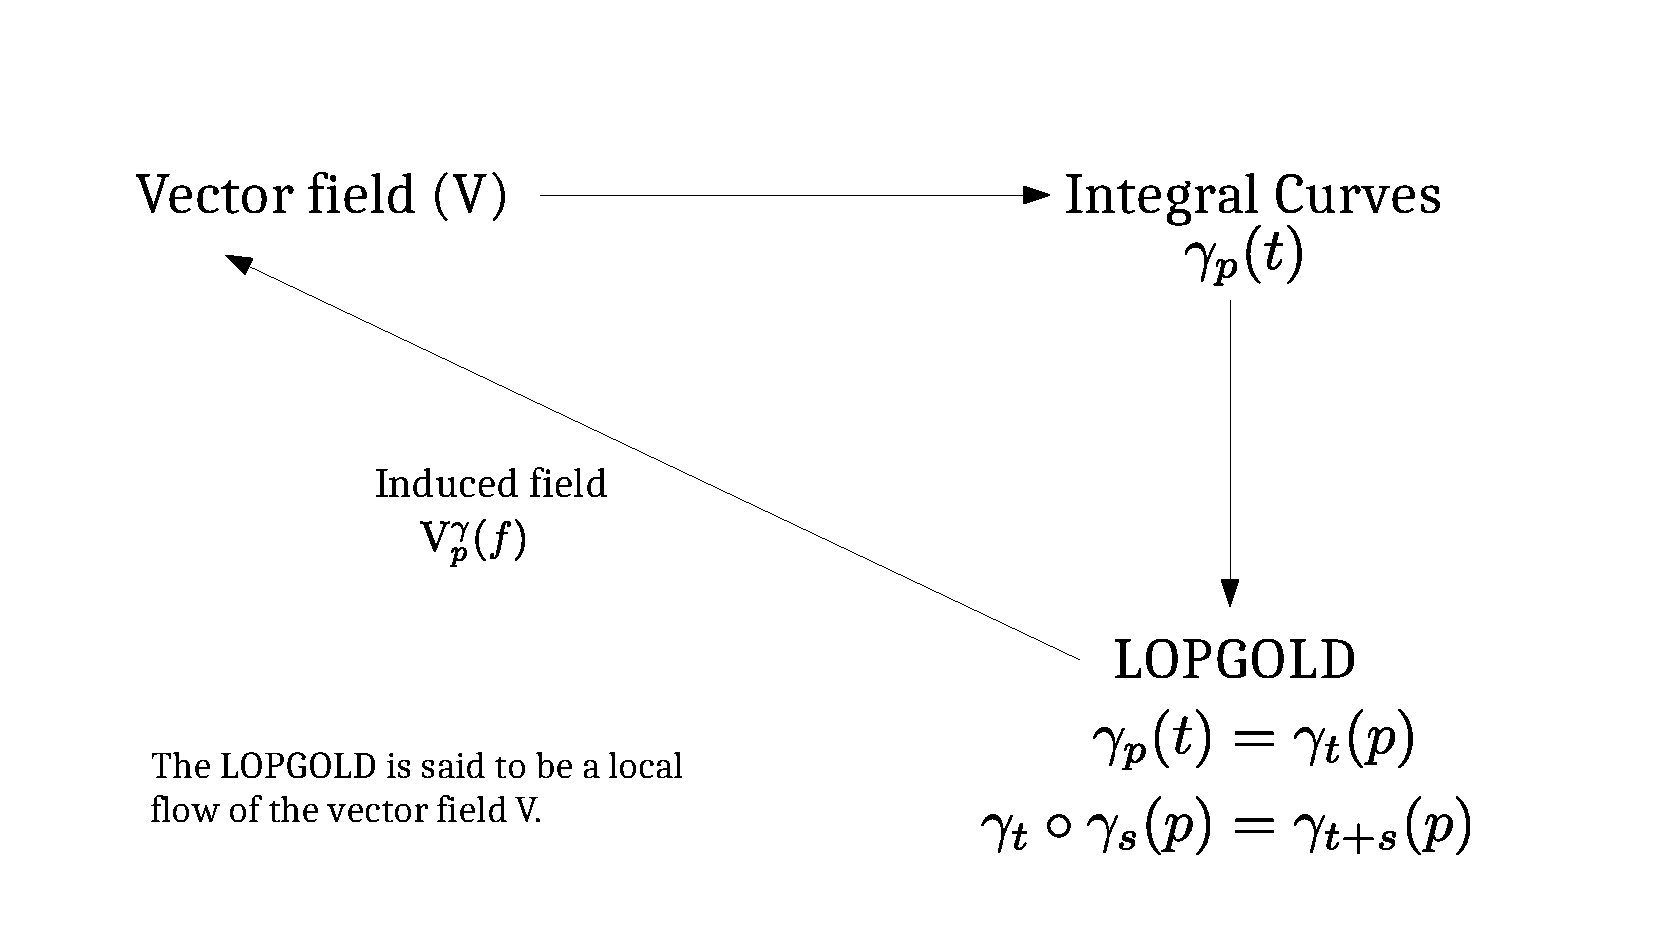
\includegraphics[width=0.8\textwidth, trim={2.3cm 1.2cm 3.1cm
      2.7cm},clip]{vectorFieldLOPGOLDIntegralCurveRelationship}
      \caption[]{}
      \label{fig: relationship between vector field, integral curve and LOPGOLD}
    \end{figure}
  \section{The Lie Derivative}
    Suppose that we have a given vector field $V$, then we know from our
    discussion above that there are local flows associated with this vector
    field. Question: if we are given another vector field $W$, then what is
    the rate of change of $W$ along the flow generated by $V$? To answer this
    question, we need the concept of the Lie derivative of a vector field:
    \begin{definition}[Lie derivative of a vector field]
      Suppose we have two vector fields $V$ and $W$. Then, we define the Lie
      derivative of $W$ with respect to $V$ by:
      \begin{equation}
        \label{eqn: Lie derivative of a vector field}
        \mathcal{L}_{V}W\bigr|_{p} = \lim_{t \rightarrow 0
        }\frac{1}{t}\left[\gamma_{-t*}W_{p'} - W_p\right]
      \end{equation}
      where $\gamma_t$ is a local flow assocaited with $V$ and $p^\prime =
      \gamma_t(p)$.
    \end{definition}
    \begin{remark}
      We can visualise equation~\ref{eqn: Lie derivative of a vector field}
      as shown in Figure~\ref{fig: Lie derivative Definition}. Essentially,
      equation~\ref{eqn: Lie derivative of a vector field} is motivated by
      the fact that we want to compare $W_{p^\prime}$ (the vector field $W$
      at the point $p^\prime$) with $W_p$ (the vector field $W$ at the point
      $p$), where $p^\prime$ is a point along the integral curve of the flow
      $\gamma_p(t)$. However, beacuse we can't compare tangent vectors
      belonging to different tangent spaces, we have to push forward
      $W_{p^\prime}$ to $T_p(\mathcal{M})$, and that is done using the push
      forward map ${\gamma_{-t}}_*$. The Lie derivative is thus the limit
      where $t \to 0$.
      \begin{figure}
        \centering
        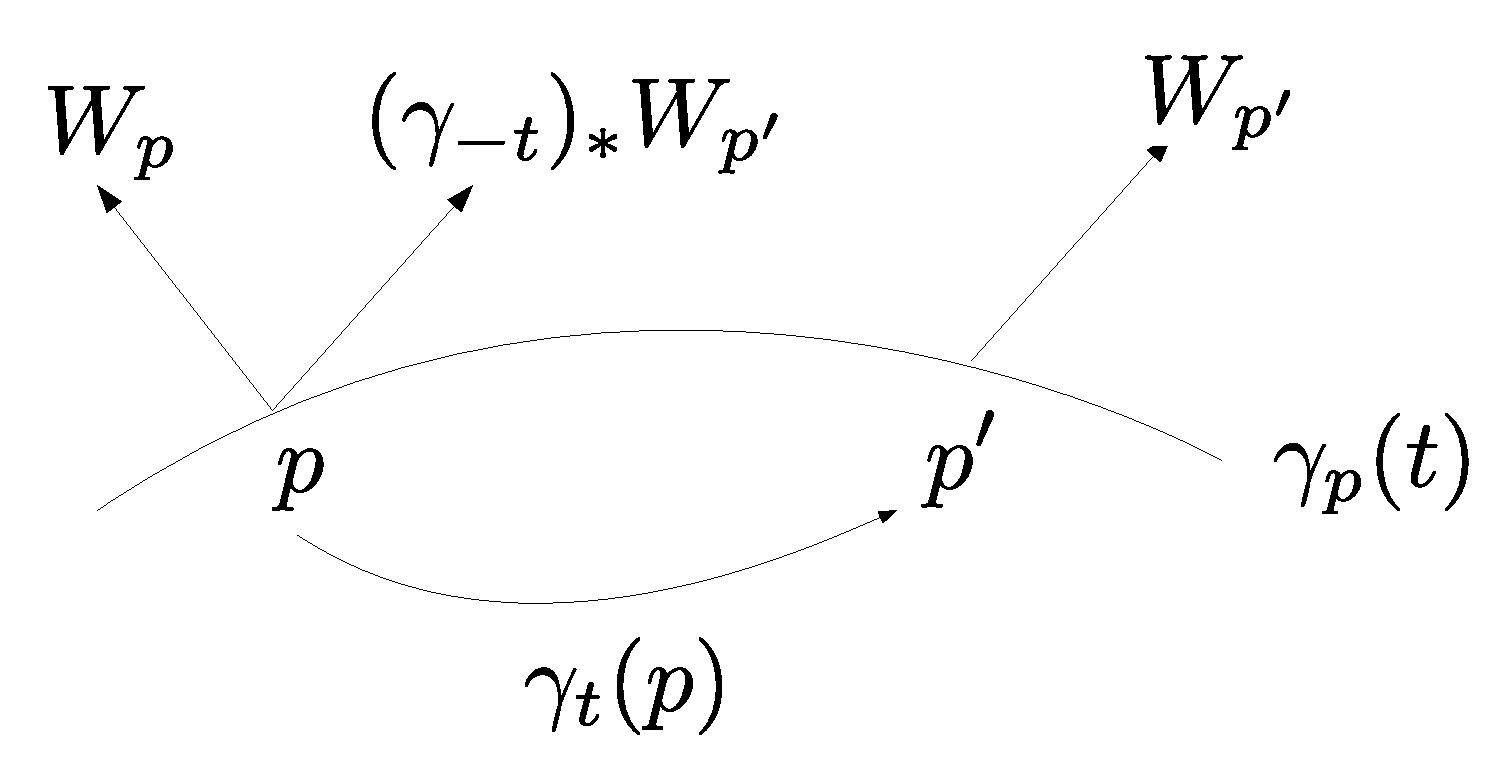
\includegraphics[width=0.6\textwidth, trim={0cm 0cm 0cm
        0cm},clip]{LieDerivativeDefn}
        \caption[]{}
        \label{fig: Lie derivative Definition}
      \end{figure}
    \end{remark}
    We can similarly define the Lie derivative of a one-form, but with the
    pull-back map rather than the push-forward map.
    \begin{definition}[Lie derivative of a one-form]
      \begin{equation}
      \label{eqn: Lie derivative of a one-form}
        \mathcal{L}_{V}\theta\bigr|_{p} = \lim_{t \rightarrow 0
        }\frac{1}{t}\left[\gamma_t^{*} \theta _{p'} - \theta_p\right]
      \end{equation}
    \end{definition}
    \begin{remark}
      Here, we have pulled-back the one-form at $p^\prime$, to the point $p$
      and subtracted $\theta_p$ from it.
    \end{remark}
    The notion of a Lie derivative can be extended to any tensor field in a
    natural way. For instance, if $\mathcal{R} \in T^{(1,1)}$, with
    $\mathcal{R} = W \otimes \theta$, where $W$ is a vector field and
    $\theta$ is a one-form, we define the Lie derivative of $\mathcal{R}$ as:
    \begin{equation}
    \label{eqn: Lie derivative of a 1-1 tensor}
      \mathcal{L}_{V}\mathcal{R}\bigr|_{p} = \lim_{t \rightarrow 0
      }\frac{1}{t}\left[\gamma_{-t*}W_{p'} \otimes \gamma_t^{*}\theta_{p'} -
      W_p \otimes \theta_p \right]
    \end{equation}
    In a similar way, we can extend the notion to any tensor field; just
    pull-back the basis one-forms, and push-forward the basis vectors.

    We note in theorem~\ref{theorem: alternate lie derivative definition}
    that the Lie derivative can be defined in other ways.
    \begin{theorem}[Alternate definitions of the Lie derivative]
      \label{theorem: alternate lie derivative definition}
      Other than equation~\ref{eqn: Lie derivative of a vector field}, the
      Lie derivative can be defined as:
      \begin{align}
        \mathcal{L}_V W\Bigr|_p 
        &= \lim_{t \to 0}[W_p - {\gamma_{t}}_*W_{\gamma_{-t}(p)}] \label{eqn:
        Lie derivative alternate defn 1}\\
        &= \lim_{t \to 0}[W_{\gamma_t(p)} - {\gamma_{t}}_*W_{p}] \label{eqn:
        Lie derivative alternate defn 2}
      \end{align}
    \end{theorem}
    \begin{remark}
      To understand equations~\ref{eqn: Lie derivative alternate defn
      1},\ref{eqn: Lie derivative alternate defn 2}, it is helpful to draw
      figures analogous to Figure~\ref{fig: Lie derivative Definition}.
      \textcolor{red}{Note to self:} These figures will be included in a
      later edition of the notes if I'm free to draw the figures...
    \end{remark}
    \subsection{Properties of Lie derivatives (part 1)}
      Here we use the definition of the Lie derivative to prove some
      properties of the Lie derivative.
        \begin{enumerate}
          \item{Given two tensor fields $R$, $S$ of the same type then:
          \begin{equation}
            \label{eqn: Lie derivative linearity}
            \mathcal{L}_V(R+S) = \mathcal{L}_V(R) + \mathcal{L}_V(S)
          \end{equation}
          \begin{proof}
            This can be shown easily through the linearity of both the
            push-forward and pull-back maps. Using $\gamma_{\pm t*}$ to denote
            both push-forward and pull-back operators respectively, we have:
            \begin{align*}
              \mathcal{L}_V(R+S)\Bigr|_p 
              &= \lim_{t\to 0}\frac{1}{t}\left[\gamma_{\pm
              t*}(R+S)_{p^\prime} - (R+S)_p\right] \\
              &= \lim_{t\to 0}\frac{1}{t}\left[\gamma_{\pm
              t*}R_{p^\prime}+\gamma_{\pm
              t*}S_{p^\prime} - R_p+S_p\right] \\
              &= \lim_{t\to 0}\frac{1}{t}\left[\gamma_{\pm t*}R_{p^\prime}-
              R_p \right]
              +\lim_{t\to 0}\frac{1}{t}\left[\gamma_{\pm
              t*}S_{p^\prime} - S_p\right] \\
              &= \mathcal{L}_V(R) + \mathcal{L}_V(S)
            \end{align*}
          \end{proof}}
          \item{For any two tensor fields $X$ and $Y$, we have:
          \begin{equation}
            \label{eqn: Lie derivative Leibniz rule}
            \mathcal{L}_V(X \otimes Y) = \mathcal{L}_V(X) \otimes Y + X
            \otimes \mathcal{L}_V(Y)
          \end{equation}
          \begin{proof}
            The proof proceeds as follows:
              \[\mathcal{L}_V(X \otimes Y) = \lim_{t \to
              0}\frac{1}{t}\left[\gamma_{\pm t*}X_{p^\prime} \otimes
              \gamma_{\pm t*}Y_{p^\prime} - X_p \otimes Y_p\right]\]
            Subtracting and adding $X_p \otimes \gamma_{\pm t*}Y_{p^\prime}$,
            we have:
            \begin{align*}
              \mathcal{L}_V(X \otimes Y)_p &=\lim_{t \to
              0}\frac{1}{t}\left[\gamma_{\pm t*}X_{p^\prime} \otimes
              \gamma_{\pm t*}Y_{p^\prime} - X_p \otimes \gamma_{\pm
              t*}Y_{p^\prime} + X_p \otimes \gamma_{\pm t*}Y_{p^\prime}- X_p
              \otimes Y_p\right] \\
              &= \lim_{t \to 0}\frac{1}{t}\left[\left(\gamma_{\pm
              t*}X_{p^\prime}- X_p \right) \otimes \gamma_{\pm
              t*}Y_{p^\prime} \right] + \lim_{t \to 0}\frac{1}{t}\left[X_p
              \otimes \left(\gamma_{\pm t*}Y_{p^\prime}-Y_p\right)\right] \\
              &= \mathcal{L}_V(X) \otimes Y\Bigr|_p + X \otimes
              \mathcal{L}_V(Y)\Bigr|_p
            \end{align*}
            which gives the desired result.
          \end{proof}}
        \end{enumerate}
    \subsection{Explicit evaluation of Lie derivatives}
      \subsubsection{Lie derivative of a 0-form (or a function)}
        First, we recall that for a general differentiable map
        $\mathcal{F}:\mathcal{M} \rightarrow \mathcal{N}$ where $\mathcal{M}$
        and $\mathcal{N}$ are two smooth manifolds, the pull-back of
        $f^\prime \in C^\infty(\mathcal{N})$ is: 
        \begin{equation}
          \label{eqn: pull-back of function}
          \mathcal{F}^{*}f^\prime =
          f^\prime \circ \mathcal{F}
        \end{equation}
         The reason for this is that we want
        $\left[\mathcal{F}^{*}f^\prime\right](p) = f^\prime(p^\prime)$, where
        $p^\prime =
        \mathcal{F}(p)$. The situation is shown in Figure~\ref{fig:
        pullBackOfFunction}.
        \begin{figure}
          \centering
          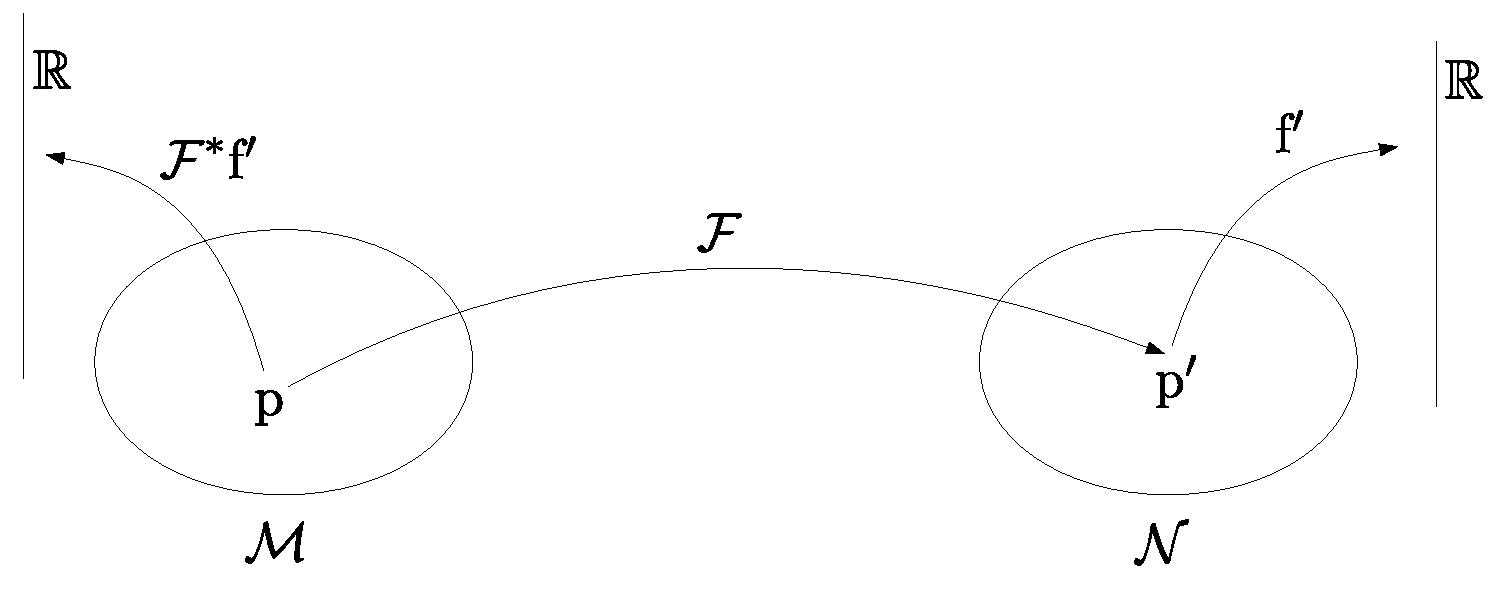
\includegraphics[width=0.75\textwidth, trim={0cm 0cm 0cm
          0cm},clip]{pullBackOfFunction}
          \caption[]{}
          \label{fig: pullBackOfFunction}
        \end{figure}
        Now, we will apply equation~\ref{eqn: pull-back of function} to the
        cases where $\mathcal{F} = \gamma_t(p)$, i.e to the case of a local
        flow. We have:
        \begin{align*}
          \mathcal{L}_V f\Bigr|_p &= \lim_{t\to 0}\frac{1}{t} \left[\gamma^*_t
          f_{p^\prime} - f_p\right] \\
          &= \lim_{t\to 0}\frac{1}{t} \left[f \circ \gamma_t(p) -
          f(p)\right] \\
          &= \lim_{t\to 0}\frac{1}{t} \left[f(\gamma_t(p)) -
          f(p)\right] \\ 
          &= \lim_{t\to 0}\frac{1}{t} \left[f(\gamma_t(p)) -
          f(\gamma_0(p))\right] \\ 
          &=\frac{d}{dt}\left[f \circ \gamma_t(p)\right]\Bigr|_{t=0} \\
          &=\frac{d}{dt}\left[f \circ \gamma_p(t)\right]\Bigr|_{t=0} \\
          &=V^\gamma_p(f) \\
          &=V_p(f)
        \end{align*}
        where to go from the second last line to the last line, we realise
        that $\gamma$ is the integral curve of $V$.

        Thus, we see that the Lie derivative of a function (or a 0-form) is
        just the directional derivative of that function.
      \subsubsection{Lie derivative of a vector field $W$}
        Now, we go back to our original scenario in equation~\ref{eqn: Lie
        derivative of a vector field}, reproduced here for convenience:
        \[\mathcal{L}_{V}W\bigr|_{p} = \lim_{t \rightarrow 0
        }\frac{1}{t}\left[\gamma_{-t*}W_{p'} - W_p\right]\]
        We shall evaluate equation~\ref{eqn: Lie derivative of a vector
        field} in a local chart $(U,\phi)$ with coordinates $\phi(p) =
        (x^1,...,x^m)$. Our strategy will be first consider $W =
        \frac{\partial}{\partial x^i}$, i.e we consider a basis field first.
        Then, we can find the expression for a general vector field.

        In the local chart $(U,\phi)$, we shall make the following
        identifications:
        \begin{gather*}
          \phi(p) = x \equiv (x^1,...,x^m)\\
          \phi(p^\prime) = y \equiv (y^1,...,y^m)\\
          \gamma_t(p) = p^\prime \xRightarrow[(U,\phi)]{\text{Local chart}}
          \overline{\gamma}_t(x) = y \\
          W_{p^\prime} \xrightarrow[(U,\phi)]{\text{Local chart}}
          \overline{W}_y \quad \quad
          W_{p} \xrightarrow[(U,\phi)]{\text{Local chart}}
          \overline{W}_x
        \end{gather*}
        Note also that since $p$ and $p^\prime$ lie on the same integral
        curve $\gamma_p(t)$, we have:
        \begin{gather*}
          \gamma_p(t) = p^\prime \xRightarrow[(U,\phi)]{\text{Local chart}}
          \overline{\gamma}_x(t) = (x^1(t),...,x^m(t)) = (y^1,...,y^m) \\
          \gamma_p(0) = p^\prime \xRightarrow[(U,\phi)]{\text{Local chart}}
          \overline{\gamma}_x(0) = (x^1(0),...,x^m(0)) = (x^1,...,x^m)
        \end{gather*}
        where the second line above is a direct consequence of the first. All
        of this is shown nicely in Figure~\ref{fig: Lie derivative of vector
        field evaluation}.
        \begin{figure}
          \centering
          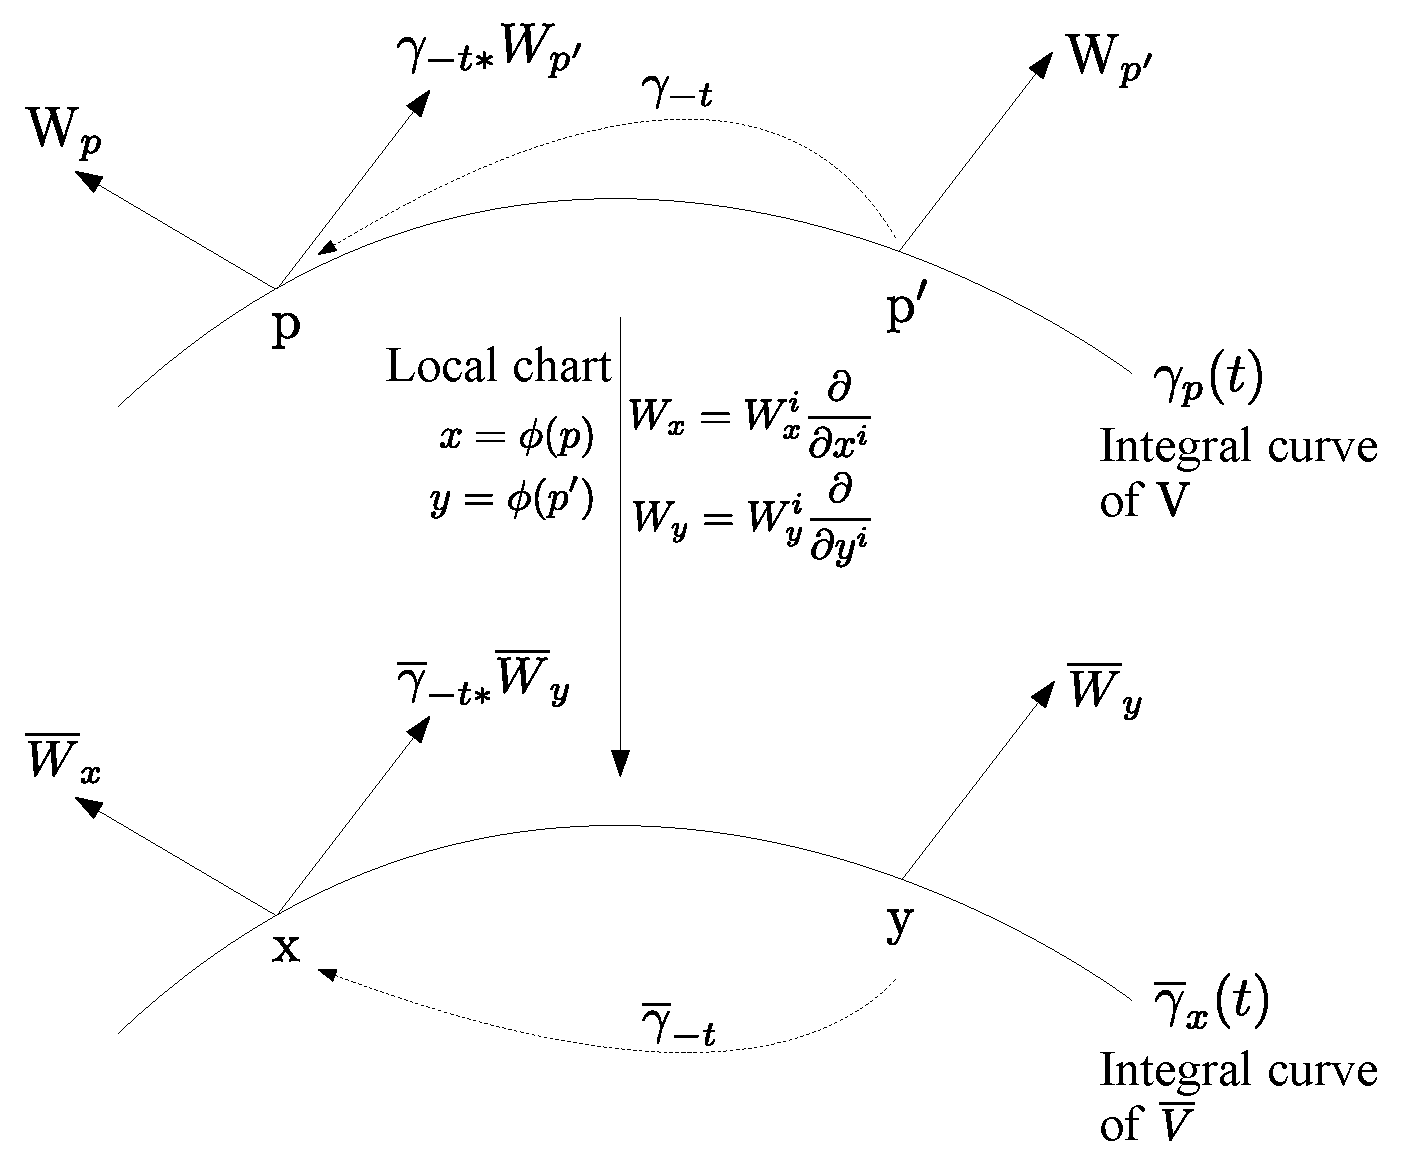
\includegraphics[width=0.8\textwidth, trim={0cm 0cm 0cm
          0cm},clip]{LieDerivativeOfVectorFieldEvaluation}
          \caption[]{}
          \label{fig: Lie derivative of vector field evaluation}
        \end{figure}
        Thus, in a local chart $(U,\phi)$, the Lie derivative definition
        looks like:
        \begin{equation}
          \label{eqn: Lie derivative vector field evaluation local chart}
          \mathcal{L}_{\overline{V}}\overline{W}\Bigr|_x = \lim_{t \to
          0}\frac{1}{t}\left[\overline{\gamma}_{-t*}\overline{W}_y -
          \overline{W}_x \right]
        \end{equation}
        Let's explicitly evaluate equation~\ref{eqn: Lie derivative vector
        field evaluation local chart} by first evaluating
        $\overline{\gamma}_{-t*}\overline{W}_y\left(\bar{f}\right)$, where
        $\bar{f} \in C^\infty(\mathbb{R})$ is a function of $x$. Now,
        \begin{align*}
          \overline{\gamma}_{-t*}\overline{W}_y\left(\bar{f}\right) 
          &= \overline{W}_y\left(\bar{f}\circ \gamma_{-t}(y)\right)
        \end{align*}
        Using the fact that according to Figure~\ref{fig: Lie derivative of
        vector field evaluation}, $\gamma_{-t}(y)$ gives us $m$ equations of
        the form $x^i = x^i(y^1,...,y^m)$, where $i = 1,..,m$, we have:
        \begin{align*}
          \overline{\gamma}_{-t*}\overline{W}_y\left(\bar{f}\right) 
          &=
          \overline{W}_y\left(\bar{f}(x^1(y^1,...,y^m),...,x^m(y^1,...,y^m))\right)
          \\
          &=
          \overline{W}^k_y\frac{\partial}{\partial
          y^k}\left(\bar{f}(x^1(y^1,...,y^m),...,x^m(y^1,...,y^m))\right) \\
          &=\overline{W}^k_y\frac{\partial \bar{f}}{\partial
          x^j}\frac{\partial x^j}{\partial y^k}\\
          &= \overline{W}^k_y\frac{\partial \bar{f}}{\partial
          x^j}\frac{\partial \overline{\gamma}_{-t}^j}{\partial y^k} \\
          &= \overline{W}^k_y\frac{\partial
          \overline{\gamma}_{-t}^j}{\partial y^k}\frac{\partial
          \bar{f}}{\partial x^j}
        \end{align*}
        Substituting the above result into equation~\ref{eqn: Lie
        derivative vector field evaluation local chart}, we have:
        \begin{align*}
          \mathcal{L}_{\overline{V}}\overline{W}\Bigr|_x \bar{f}
          &= \lim_{t \to
          0}\frac{1}{t}\left[\overline{\gamma}_{-t*}\overline{W}_y -
          \overline{W}_x \right]\left(\bar{f}\right) \\
          &= \lim_{t \to
          0}\frac{1}{t}\left[ \overline{W}^k_y\frac{\partial
          \overline{\gamma}_{-t}^j}{\partial y^k}\frac{\partial
          \bar{f}}{\partial x^j} -
          \overline{W}^k_x\frac{\partial \bar{f}}{\partial x^k} \right]
        \end{align*}
        Now, we restrict ourselves to the basis field $\overline{W} =
        \dfrac{\partial}{\partial x^i}$, which gives us:
        \[\overline{W}_x^k =\overline{W}_x^k = \delta^k_i \]
        Then, we have:
        \begin{align*}
          \mathcal{L}_{\overline{V}}\left(\frac{\partial}{\partial
          x^i}\right)\Bigr|_x \bar{f}
          &= \lim_{t \to 0}\frac{1}{t}\left[ \delta^k_i \frac{\partial
          \overline{\gamma}_{-t}^j}{\partial y^k}\frac{\partial
          \bar{f}}{\partial x^j} - \delta^k_i\frac{\partial \bar{f}}{\partial
          x^k} \right] \\
          &= \lim_{t \to 0}\frac{1}{t}\left[\frac{\partial
          \overline{\gamma}_{-t}^j}{\partial y^i}\frac{\partial
          \bar{f}}{\partial x^j} - \delta^k_i\frac{\partial \bar{f}}{\partial
          x^k} \right]
        \end{align*}
        Using some mathematical trickery, i.e $\delta_i^k = \dfrac{\partial
        y^k}{\partial y^i}$, we have:
        \begin{align*}
          \mathcal{L}_{\overline{V}}\left(\frac{\partial}{\partial
          x^i}\right)\Bigr|_x \bar{f}
          &= \lim_{t \to 0}\frac{1}{t}\left[\frac{\partial
          \overline{\gamma}_{-t}^j}{\partial y^i}\frac{\partial
          \bar{f}}{\partial x^j} - \frac{\partial y^k}{\partial
          y^i}\frac{\partial \bar{f}}{\partial x^k} \right]\\
          &= \lim_{t \to 0}\frac{1}{t}\left[\frac{\partial
          \overline{\gamma}_{-t}^j}{\partial y^i}\frac{\partial
          \bar{f}}{\partial x^j} - \frac{\partial
          \overline{\gamma}^j_{0}}{\partial y^i}\frac{\partial
          \bar{f}}{\partial x^j} \right] \\
        \end{align*}
        where we note that $\gamma_0$ is the identity map, i.e $\gamma_0(y) =
        y$. Making the $y$ dependence of $\gamma_{-t}^j$ explicit, we
        have\footnote{The derivation from here onwards departs from Kuldip's
        treatment, not sure how legit it is. The departure is because
        Kuldip's treatment seems sketchy...}:
        \begin{align*}
          \mathcal{L}_{\overline{V}}\left(\frac{\partial}{\partial
          x^i}\right)\Bigr|_x \bar{f}
          &= \lim_{t \to 0}\frac{1}{t}\left[\frac{\partial
          \overline{\gamma}_{-t}^j(y^1,...,y^m)}{\partial
          y^i}\frac{\partial \bar{f}}{\partial x^j} -
          \frac{\partial
          \overline{\gamma}^j_{0}(y^1,...,y^m)}{\partial
          y^i}\frac{\partial \bar{f}}{\partial x^j} \right] \\
          &= \lim_{t \to 0}\frac{1}{t}\left[\frac{\partial
          \overline{\gamma}_{-t}^j(y^1,...,y^m)}{\partial y^i} -
          \frac{\partial \overline{\gamma}^j_{0}(y^1,...,y^m)}{\partial y^i}
          \right]\frac{\partial \bar{f}}{\partial x^j}
        \end{align*}
        Now, making the substitution $s = -t$, we have:
        \begin{align*}
          \mathcal{L}_{\overline{V}}\left(\frac{\partial}{\partial
          x^i}\right)\Bigr|_x \bar{f}
          &= -\lim_{s \to 0}\frac{1}{s}\left[\frac{\partial
          \overline{\gamma}_{s}^j(y^1,...,y^m)}{\partial y^i} -
          \frac{\partial \overline{\gamma}^j_{0}(y^1,...,y^m)}{\partial
          y^i}\right] \frac{\partial \bar{f}}{\partial x^j} \\
          &= -\lim_{s \to 0}\left[\frac{\partial}{\partial
          y^i}\left(\frac{\overline{\gamma}_{s}^j(y^1,...,y^m) -
          \overline{\gamma}_{0}^j(y^1,...,y^m)}{s}\right)
          \right]\frac{\partial \bar{f}}{\partial x^j}
        \end{align*}
        Now, the limit in the last line above is a tricky limit to take. We
        first realise that $s \to 0 \implies t \to 0$, and $t \to 0 \implies
        y \to x$. Thus, this allows us to do:
        \begin{align*}
          \mathcal{L}_{\overline{V}}\left(\frac{\partial}{\partial
          x^i}\right)\Bigr|_x \bar{f}
          &= -\lim_{s \to 0}\left[\frac{\partial}{\partial
          x^i}\left(\frac{\overline{\gamma}_{s}^j(x^1,...,x^m) -
          \overline{\gamma}_{0}^j(x^1,...,x^m)}{s}\right)
          \right]\frac{\partial \bar{f}}{\partial x^j}
        \end{align*}
        which then gives us:
        \begin{align*}
          \mathcal{L}_{\overline{V}}\left(\frac{\partial}{\partial
          x^i}\right)\Bigr|_x \bar{f} 
          &= -\frac{\partial}{\partial x^i}\left(\frac{d
          \overline{\gamma}_s^j(x^1,...,x^m)}{ds}\Bigr|_{s=0}\right)
          \frac{\partial \bar{f}}{\partial x^j} \\
          &= -\frac{\partial}{\partial x^i}\left(\frac{d
          \overline{\gamma}_x^j(s)}{ds}\Bigr|_{s=0}\right)
          \frac{\partial \bar{f}}{\partial x^j}
        \end{align*}
        Realising that $\dfrac{d \overline{\gamma}_x^j(s)}{ds}$ is $j$-th
        component of the tangent vector to the integral curve at the point
        $x$, which is just another way to refer to the $j$-th component of
        the vector field $\overline{V}_x$, we have:
        \begin{equation}
          \label{eqn: Lie derivative of basis field}
          \mathcal{L}_{\overline{V}}\left(\frac{\partial}{\partial
          x^i}\right)\Bigr|_x = -\frac{\partial}{\partial
          x^i}\left(\overline{V}^j_x\right) \frac{\partial \bar{f}}{\partial
          x^j}
        \end{equation}
        Now that we have equation~\ref{eqn: Lie derivative of basis field},
        we can easily extend our results to include any field $\overline{W} =
        \overline{W}^i\dfrac{\partial}{\partial x^i}$ using
        equation~\ref{eqn: Lie derivative linearity} and equation~\ref{eqn:
        Lie derivative Leibniz rule}. I.e, we can write:
        \begin{align*}
          \overline{W} &= \overline{W}^i\dfrac{\partial}{\partial x^i} \\ 
          &= \overline{W}^1\frac{\partial}{\partial x^1} +
          \overline{W}^2\frac{\partial}{\partial x^2} + ... +
          \overline{W}^m\dfrac{\partial}{\partial x^m}
        \end{align*}
        which gives us
        \begin{align*}
          \mathcal{L}_{\overline{V}}\overline{W}
          &=
          \mathcal{L}_{\overline{V}}\left(\overline{W}^i\frac{\partial}{\partial
          x^i}\right) \\
          &=
          \mathcal{L}_{\overline{V}}\left(\overline{W}^1\frac{\partial}{\partial
          x^1}\right) +
          \mathcal{L}_{\overline{V}}\left(\overline{W}^2\frac{\partial}{\partial
          x^2}\right) + ... +
          \mathcal{L}_{\overline{V}}\left(\overline{W}^m\dfrac{\partial}{\partial
          x^m}\right)
        \end{align*}
        and note that for each individual term in the summation, say
        $\mathcal{L}_{\overline{V}}\left(\overline{W}^1\dfrac{\partial}{\partial
        x^1}\right)$, we can treat $\overline{W}^1$ as a 0-form and
        $\dfrac{\partial}{\partial x^1}$ as a vector and then apply
        equation~\ref{eqn: Lie derivative Leibniz rule}. E.g:
        \begin{align*}
          \mathcal{L}_{\overline{V}}\left(\overline{W}^1\frac{\partial}{\partial
          x^1}\right)
          &=
          \mathcal{L}_{\overline{V}}\left(\overline{W}^1\right) +
          \frac{\partial}{\partial
          x^1}
          \overline{W}^1\mathcal{L}_{\overline{V}}\left(\frac{\partial}{\partial
          x^1}\right) \\
          &= V^j \frac{\partial \overline{W}^1}{\partial
          x^j}\frac{\partial}{\partial x^1} + \overline{W}^1
          \left(-\frac{\partial}{\partial x^1}\left(\overline{V}^j\right)
          \frac{\partial}{\partial x^j}\right) \\
          &= V^j\frac{\partial \overline{W}^1}{\partial
          x^j}\frac{\partial}{\partial x^1} - \overline{W}^1 \frac{\partial
          \overline{V}^j}{\partial x^1}\frac{\partial}{\partial x^j}
        \end{align*}
        Thus, summing over all these individual terms, we have:
        \begin{align*}
          \mathcal{L}_{\overline{V}}\left(\overline{W}^i\frac{\partial}{\partial
          x^i}\right) &=
          V^j\frac{\partial \overline{W}^i}{\partial
          x^j}\frac{\partial}{\partial x^i} - \overline{W}^i \frac{\partial
          \overline{V}^j}{\partial x^i}\frac{\partial}{\partial x^j}
        \end{align*}
        Doing a renaming of dummy variables for the first term, i.e the good
        old $ i\leftrightarrow j$, we have:
        \begin{align*}
          \mathcal{L}_{\overline{V}}\left(\overline{W}^i\frac{\partial}{\partial
          x^i}\right) 
          &= V^i\frac{\partial \overline{W}^j}{\partial
          x^i}\frac{\partial}{\partial x^j} - \overline{W}^i \frac{\partial
          \overline{V}^j}{\partial x^i}\frac{\partial}{\partial x^j} \\
          &=\left(V^i\frac{\partial \overline{W}^j}{\partial x^i} -
          \overline{W}^i \frac{\partial \overline{V}^j}{\partial x^i}
          \right)\frac{\partial}{\partial x^j}
        \end{align*}
        With reference to equation~\ref{eqn: commutator in local chart},
        notice that the last line is exactly how the the commutator of
        $\overline{V}$ and $\overline{W}$ looks like. This gives us our very
        interesting result:
        \begin{equation}
          \mathcal{L}_{\overline{V}}\overline{W} =
          \left[\overline{V},\overline{W}\right]
        \end{equation}
        and this is the reason why the commutator is also called the Lie
        bracket.
      \subsubsection{Lie derivative of a one-form}
        Here, we want to evaluate equation~\ref{eqn: Lie derivative of a
        one-form} in a local chart $(U,\phi)$, which we will write as:
        \begin{equation}
          \label{eqn: Lie derivative one-form local chart}
          \mathcal{L}_{\overline{V}} \overline{\theta} = \lim_{t\to
          0}\frac{1}{t}\left[\overline{\gamma}_t^* \overline{\theta}_y -
          \overline{\theta}_x\right]
        \end{equation}
        To get from equation~\ref{eqn: Lie derivative of a one-form} to
        equation~\ref{eqn: Lie derivative one-form local chart}, we have made
        the folllowing substitutions:
        \begin{align*}
          \phi(p) = x, &\quad \quad \quad \quad \phi(p^\prime) = y \\
          p^\prime = \gamma_t(p) &\xRightarrow[(U,\phi)]{\text{Local Chart}}
          y = \gamma_t(x)\\
          \theta_{p^\prime} &\xrightarrow[(U,\phi)]{\text{Local Chart}}
          \overline{\theta}_y \\
          \theta_{p} &\xrightarrow[(U,\phi)]{\text{Local Chart}}
          \overline{\theta}_x
        \end{align*}
        Note that the second equation above gives us $m$ coordinate
        transformation equations of the form: $y^i = y^i(x^1,...,x^m)$ for $i
        = 1,2,...,m$. Now, we first evaluate the $\overline{\gamma}_t^*
        \overline{\theta}_y$ term. We first have:
        \begin{align*}
          \left\langle \overline{\gamma}_t^* \overline{\theta}_y, \,
          \frac{\partial}{\partial x^i} \right\rangle
          &= \left\langle  \overline{\theta}_y, \,
          {\overline{\gamma}_t}_*\frac{\partial}{\partial x^i} \right\rangle
        \end{align*}
        Next, we note that, for $\bar{f}^\prime \in C^\infty(\mathcal{M})$
        where $\bar{f}^\prime$ is a function of $y$, we have, using
        theorem~\ref{theorem: f-related field calculation},
        \begin{align*}
          \left[{\overline{\gamma}_t}_*\frac{\partial}{\partial x^i}
          \bar{f}^\prime\right](y) 
          &= \frac{\partial}{\partial x^i}\left(\bar{f}^\prime \circ
          \overline{\gamma}_t(x^1,...,x^m) \right) \\
          &= \frac{\partial \bar{f}^\prime\left(
          \overline{\gamma}_t(x^1,...,x^m) \right)}{\partial x^i} \\
          &= \frac{\partial \bar{f}^\prime\left(
          y^1(x^1,...,x^m),...,y^m(x^1,...,x^m) \right)}{\partial x^i}\\
          &= \frac{\partial \bar{f}^\prime}{\partial y^j}\frac{\partial
          y^j}{\partial x^i}
        \end{align*}
        Noting that $\dfrac{\partial y^j}{\partial x^i} = \dfrac{\partial
        \overline{\gamma}_t^j(x^1,...,x^m)}{\partial x^i}$, our result above
        becomes:
        \[\left[{\overline{\gamma}_t}_*\frac{\partial}{\partial x^i}
        \bar{f}^\prime\right](y) = \frac{\partial
        \overline{\gamma}_t^j(x^1,...,x^m)}{\partial x^i}\frac{\partial
        \bar{f}^\prime}{\partial y^j}\]
        which gives us:
        \[{\overline{\gamma}_t}_*\frac{\partial}{\partial x^i} =
        \frac{\partial \overline{\gamma}_t^j(x^1,...,x^m)}{\partial
        x^i}\frac{\partial }{\partial y^j}\]
        Continuing with our evaluation of $\overline{\gamma}_t^*
        \overline{\theta}_y$, we have:
        \begin{align*}
          \left\langle \overline{\gamma}_t^* \overline{\theta}_y, \,
          \frac{\partial}{\partial x^i} \right\rangle
          &= \left\langle  \overline{\theta}_y, \,
          {\overline{\gamma}_t}_*\frac{\partial}{\partial x^i} \right\rangle \\
          &=\left\langle\overline{\theta}_y, \,\frac{\partial
          \overline{\gamma}_t^j(x^1,...,x^m)}{\partial x^i}\frac{\partial
          }{\partial y^j} \right\rangle \\
          &= \frac{\partial \overline{\gamma}_t^j(x^1,...,x^m)}{\partial
          x^i}\left\langle\overline{\theta}_y, \,\frac{\partial }{\partial
          y^j} \right\rangle \\
          &= \frac{\partial \overline{\gamma}_t^j(x^1,...,x^m)}{\partial
          x^i} \left(\overline{\theta}_y\right)_j \\
          &=\frac{\partial \overline{\gamma}_x^j(t)}{\partial
          x^i} \left(\overline{\theta}_y\right)_j
        \end{align*}
        where in the last line, we note that for a local flow
        $\overline{\gamma}_t$, we have $\overline{\gamma}_t(x) =
        \overline{\gamma}_x(t)$. Thus, this gives us: \[\overline{\gamma}_t^*
        \overline{\theta}_y = \frac{\partial
        \overline{\gamma}_x^j(t)}{\partial x^i}
        \left(\overline{\theta}_y\right)_j dx^i \]
        Substituting the above result into equation~\ref{eqn: Lie derivative
        one-form local chart}, we have:
        \begin{align*}
          \mathcal{L}_{\overline{V}} \overline{\theta} &= \lim_{t\to
          0}\frac{1}{t}\left[\overline{\gamma}_t^* \overline{\theta}_y -
          \overline{\theta}_x\right] \\ &=\lim_{t\to
          0}\frac{1}{t}\left[\frac{\partial
          \overline{\gamma}_x^j(t)}{\partial x^i}
          \left(\overline{\theta}_y\right)_j dx^i -
          \left(\overline{\theta}_x\right)_i dx^i\right]
        \end{align*}
        Now, we first consider a basis one-form, i.e we consider
        $\overline{\theta} = \delta_i^k dx^i = dx^k$. Then, we have:
        \begin{align*}
          \mathcal{L}_{\overline{V}} dx^k &=\lim_{t\to
          0}\frac{1}{t}\left[\frac{\partial
          \overline{\gamma}_x^j(t)}{\partial x^i} \delta_j^k dx^i -
          \delta_i^k dx^i\right] \\
          &=\lim_{t\to 0}\frac{1}{t}\left[\frac{\partial
          \overline{\gamma}_x^k(t)}{\partial x^i} dx^i - \frac{\partial
          x^k}{\partial x^i} dx^i\right] \\
          &=\lim_{t\to 0}\frac{1}{t}\left[\frac{\partial
          \overline{\gamma}_x^k(t)}{\partial x^i} dx^i - \frac{\partial
          \overline{\gamma}^k_x(0)}{\partial x^i} dx^i\right] \\
          &=\lim_{t\to 0}\frac{1}{t}\left[\frac{\partial
          \overline{\gamma}_x^k(t)}{\partial x^i} - \frac{\partial
          \overline{\gamma}^k_x(0)}{\partial x^i} \right] dx^i \\
          &=\lim_{t\to 0} \frac{\partial}{\partial
          x^i}\left[\frac{\gamma_x^k(t) - \gamma_x^k(0)}{t}\right] dx^i \\
          &=\frac{\partial}{\partial
          x^i}\left(\frac{d\overline{\gamma}_x^k}{dt}\right)\Biggr|_{t=0}
          dx^i
        \end{align*}
        Noting that $\dfrac{\partial}{\partial
        x^i}\left(\frac{d\overline{\gamma}_x^k}{dt}\right)\Biggr|_{t=0}$ is
        nothing more than the $k$-th component of the tangent vector to the
        integral curve $\gamma_x(t)$, which is the $k$-th component of the
        vector field $\overline{V}$ at $x$, we have:
        \begin{align}
        \mathcal{L}_{\overline{V}} dx^k 
        &=\frac{\partial}{\partial x^i}\left(V^k_x\right) dx^i \nonumber\\
        &=\frac{\partial V^k}{\partial x^i}dx^i
        \end{align}
        The equation above can then be used to evaluate the Lie derivative of
        any arbitrary one-form $\theta_i dx^i$, using both equation~\ref{eqn:
        Lie derivative linearity} and equation~\ref{eqn: Lie derivative
        Leibniz rule}. \textcolor{red}{This is left as an exercise
        to...future KH or whoever reads this notes}\footnote{This exercise is
        rather simple, just follow the same steps as when finding the Lie
        derivative of an arbitary vector field given the Lie derivative of
        the basis vector.}.

        Now, we shall state one very important result in the evaluation of
        Lie derivatives:
        \begin{theorem}
          \label{theorem: Lie derivative of one form theorem}
          In a local chart, for a vector field $\overline{V}$ and a one-form
          $\overline{\omega}$ we have:
          \begin{equation}
            \mathcal{L}_{\overline{V}}\overline{\omega} =
            d\left(\overline{\omega}(\overline{V})\right) +
            (d\overline{\omega})(\overline{V})
          \end{equation}
          where $d$ stands for the exterior derivative operator\footnote{To
          be introduced in a later chapter.}.
        \end{theorem}
        \begin{proof}
          \textcolor{red}{To fill in next time}
        \end{proof}
        \begin{remark}
          According to Kuldip's lecture notes, theorem~\ref{theorem: Lie
          derivative of one form theorem} holds for $2$-forms too. I wonder
          if it holds for $n$ forms; \textcolor{red}{we can try to prove this
          next time.}
        \end{remark}
    \subsection{Properties of the Lie derivative (Part 2)}
      Now that we can explicitly evaluate the Lie derivative for a scalar
      field, vector field and one-form, we can show that for a tensor $T$ in
      general, the following two properties are true:
      \begin{subequations}
        \label{eqn: Two other properties of Lie derivatives (for Lie Algebra)}
        \begin{gather}
          \mathcal{L}_{a V + b W}T = a\mathcal{L}_V T + b\mathcal{L}_W T \\
          \mathcal{L}_{[V,W]}T = \mathcal{L}_V\left(\mathcal{L}_W(T)\right)
          -\mathcal{L}_W\left(\mathcal{L}_V(T) \right)
        \end{gather}
    \end{subequations}
      \begin{proof}[Rough sketch of a proof for now]
        Since an arbitrary tensor is just of the form $T =
        T_{abc...}^{def...} \partial_d \otimes \partial_e \otimes \partial_f
        \otimes dx^a \otimes dx^b \otimes dx^c$, we can first prove these two
        equations individually for a scalar field, vector field and for a
        one-form (\textcolor{red}{To be done in the
        future\footnote{Alternatively, see Edward Teo's PC4274 tutorial
        3}.}), then apply equation~\ref{eqn: Lie derivative linearity} and
        equation~\ref{eqn: Lie derivative Leibniz rule}.
      \end{proof}
      Now, the above two properties naturally lead us to the notion of Lie
      algebras. But first, let us define what an invariant tensor field is
      first.
      \begin{definition}[Invariant tensor field]
        A tensor field $T$ is said to be invariant under a vector field $V$ if
        \[\mathcal{L}_V(T) = 0\]
        We sometimes also say that $T$ is Lie-dragged by $V$.
      \end{definition}
      \begin{remark}
        In other words, this means that as we move along the local flow
        generated by the vector field $V$, the tensor $T$ remains unchanged.
      \end{remark}
      Now, equation~\ref{eqn: Two other properties of Lie derivatives (for
      Lie Algebra)} implies that when $T$ is invariant under $V$ and $W$,
      then it is invariant under $aV+bW$ and $[V,W]$. We say that the set of
      all fields which $T$ is invariant under forms a Lie algebra. This shows
      the intimate relationship beween invariances (or symmetries) and Lie
      algebras. This idea will be explored further in a later chapter on Lie
      algebras.
    \subsection{Lie derivative and the coordinate basis}
      See Edward teo's notes chapter 3 for now, \textcolor{red}{Will add
      later when I have time.}